\documentclass[11pt]{article}

% basic packages
\usepackage[margin=1in]{geometry}
\usepackage[pdftex]{graphicx}
\usepackage{amsmath,amssymb,amsthm}
\usepackage{custom}
\usepackage{lipsum}

\usepackage{xcolor}
\usepackage{tikz-cd}

\usepackage[most]{tcolorbox}
\usepackage{xcolor}
\usepackage{mdframed}
\usepackage{calligra}


% page formatting
\usepackage{fancyhdr}
\pagestyle{fancy}

\renewcommand{\sectionmark}[1]{\markright{\textsf{\arabic{section}. #1}}}
\renewcommand{\subsectionmark}[1]{}
\lhead{\textbf{\thepage} \ \ \nouppercase{\rightmark}}
\chead{}
\rhead{}
\lfoot{}
\cfoot{}
\rfoot{}
\setlength{\headheight}{14pt}

\linespread{1.03} % give a little extra room
\setlength{\parindent}{0.2in} % reduce paragraph indent a bit
\setcounter{secnumdepth}{2} % no numbered subsubsections
\setcounter{tocdepth}{2} % no subsubsections in ToC

\DeclareMathAlphabet{\mathcalligra}{T1}{calligra}{m}{n}
\DeclareFontShape{T1}{calligra}{m}{n}{<->s*[2.2]callig15}{}
\newcommand{\scriptr}{\mathcalligra{r}\,}
\newcommand{\boldscriptr}{\pmb{\mathcalligra{r}}\,}


%%%%%%%%%%%%%%%%%%%%%%%%%%%%%%%%%%%%%%%%%%%%%%%%%%%%%%%%%%%%%%%%%
% CUSTOM BOXES AND STUFF
\newtcolorbox{redbox}{colback=red!5!white,colframe=red!75!black, breakable}
\newtcolorbox{bluebox}{colback=blue!5!white,colframe=blue!75!black, breakable}

\definecolor{lightblue}{RGB}{173,216,230} % Light blue color
\definecolor{darkblue}{RGB}{0,0,139} % Dark blue color

% Define the custom proof environment
\newtcolorbox{ex}[2][Example]{
  colback=red!5!white, % Light blue background
  colframe=red!75!black, % Darker blue border
  coltitle=white, % Title color
  fonttitle=\bfseries, % Title font style
  title={{#2}},
  arc=1mm, % Rounded corners with 4mm radius,
  boxrule=0.5mm,
  left=2mm, right=2mm, top=2mm, bottom=2mm, % Padding inside the box
  breakable, % Allow box to be broken across pages
  before=\vspace{10pt}, % Padding above the box
  after=\vspace{10pt}, % Padding below the box
  before upper={\parindent15pt} % Ensure indentation
}

% Define the custom proof environment
\newtcolorbox{defn}[2][Definition]{
  colback=blue!5!white, % Light blue background
  colframe=blue!75!black, % Darker blue border
  coltitle=white, % Title color
  fonttitle=\bfseries, % Title font style
  title={{#2}},
  arc=1mm, % Rounded corners with 4mm radius,
  boxrule=0.5mm,
  left=2mm, right=2mm, top=2mm, bottom=2mm, % Padding inside the box
  breakable, % Allow box to be broken across pages
  before=\vspace{10pt}, % Padding above the box
  after=\vspace{10pt}, % Padding below the box
  before upper={\parindent15pt} % Ensure indentation
}


%%%%%%%%%%%%%%%%%%%%%%%%%%%%%%%%%%%%%%%%%%%%%%%%%%%%%%%%%%%%%%%%%


\begin{document}

% make title page
\thispagestyle{empty}
\bigskip \
\vspace{0.1cm}

\begin{center}
{\fontsize{22}{22} \selectfont (Instructor: James Analytis)}
\vskip 16pt
{\fontsize{36}{36} \selectfont \bf \sffamily Physics 141B: Introduction to Solid State II Notes}
\vskip 24pt
{\fontsize{18}{18} \selectfont \rmfamily Keshav Balwant Deoskar} 
\vskip 6pt
{\fontsize{14}{14} \selectfont \ttfamily kdeoskar@berkeley.edu} 
\vskip 24pt
\end{center}

% {\parindent0pt \baselineskip=15.5pt \lipsum[1-4]} 

% make table of contents
% \newpage

These are some notes taken from UC Berkeley's Physics 141B during the Fall '24 session, taught by James Analytis. This template is based heavily off of the one produced by \href{https://knzhou.github.io/}{Kevin Zhou}.

% \microtoc
\tableofcontents 


%%%%%%%%%%%%%%%%%%%%%%%%%%%%%%%%%%%%%%%%%%%%%%%%
\pagebreak
\section{January 22, 2025:}
%%%%%%%%%%%%%%%%%%%%%%%%%%%%%%%%%%%%%%%%%%%%%%%%

Office Hours Fri 1-2pm after Lecture.\\
Syllabus: 
\begin{itemize}
  \item Topology: (6-7 weeks)
  \begin{itemize}
    \item Su-Shrieffer-Heeger Model
    \item Berry's Phase and its application to Graphene
    \item Haldane Model
    \item Topological Insulators
  \end{itemize}

  \item Superconductivity: (3-4 weeks)
  \begin{itemize}
    \item Overview and Two-fluid Model
    \item Cooper pairing
    \item Bardeen, Cooper, Schrieffer (BCS) Model
    \item Josephson Effect
  \end{itemize}

  \item If we have time, Magnetism: 
  \begin{itemize}
    \item Phenomenology, Ferromagnets and Antiferromagnets
    \item Direct-exchange and Super-exchange
    \item Mean-field Model
  \end{itemize}
\end{itemize}

\vskip 1cm
\subsection{Review: The Tight Binding model}
Consider a 1D Chain of $N$ sites with 1 orbital per site, and consider a unit cell with 1 site per cell defined as in the picture below:
\begin{center}
  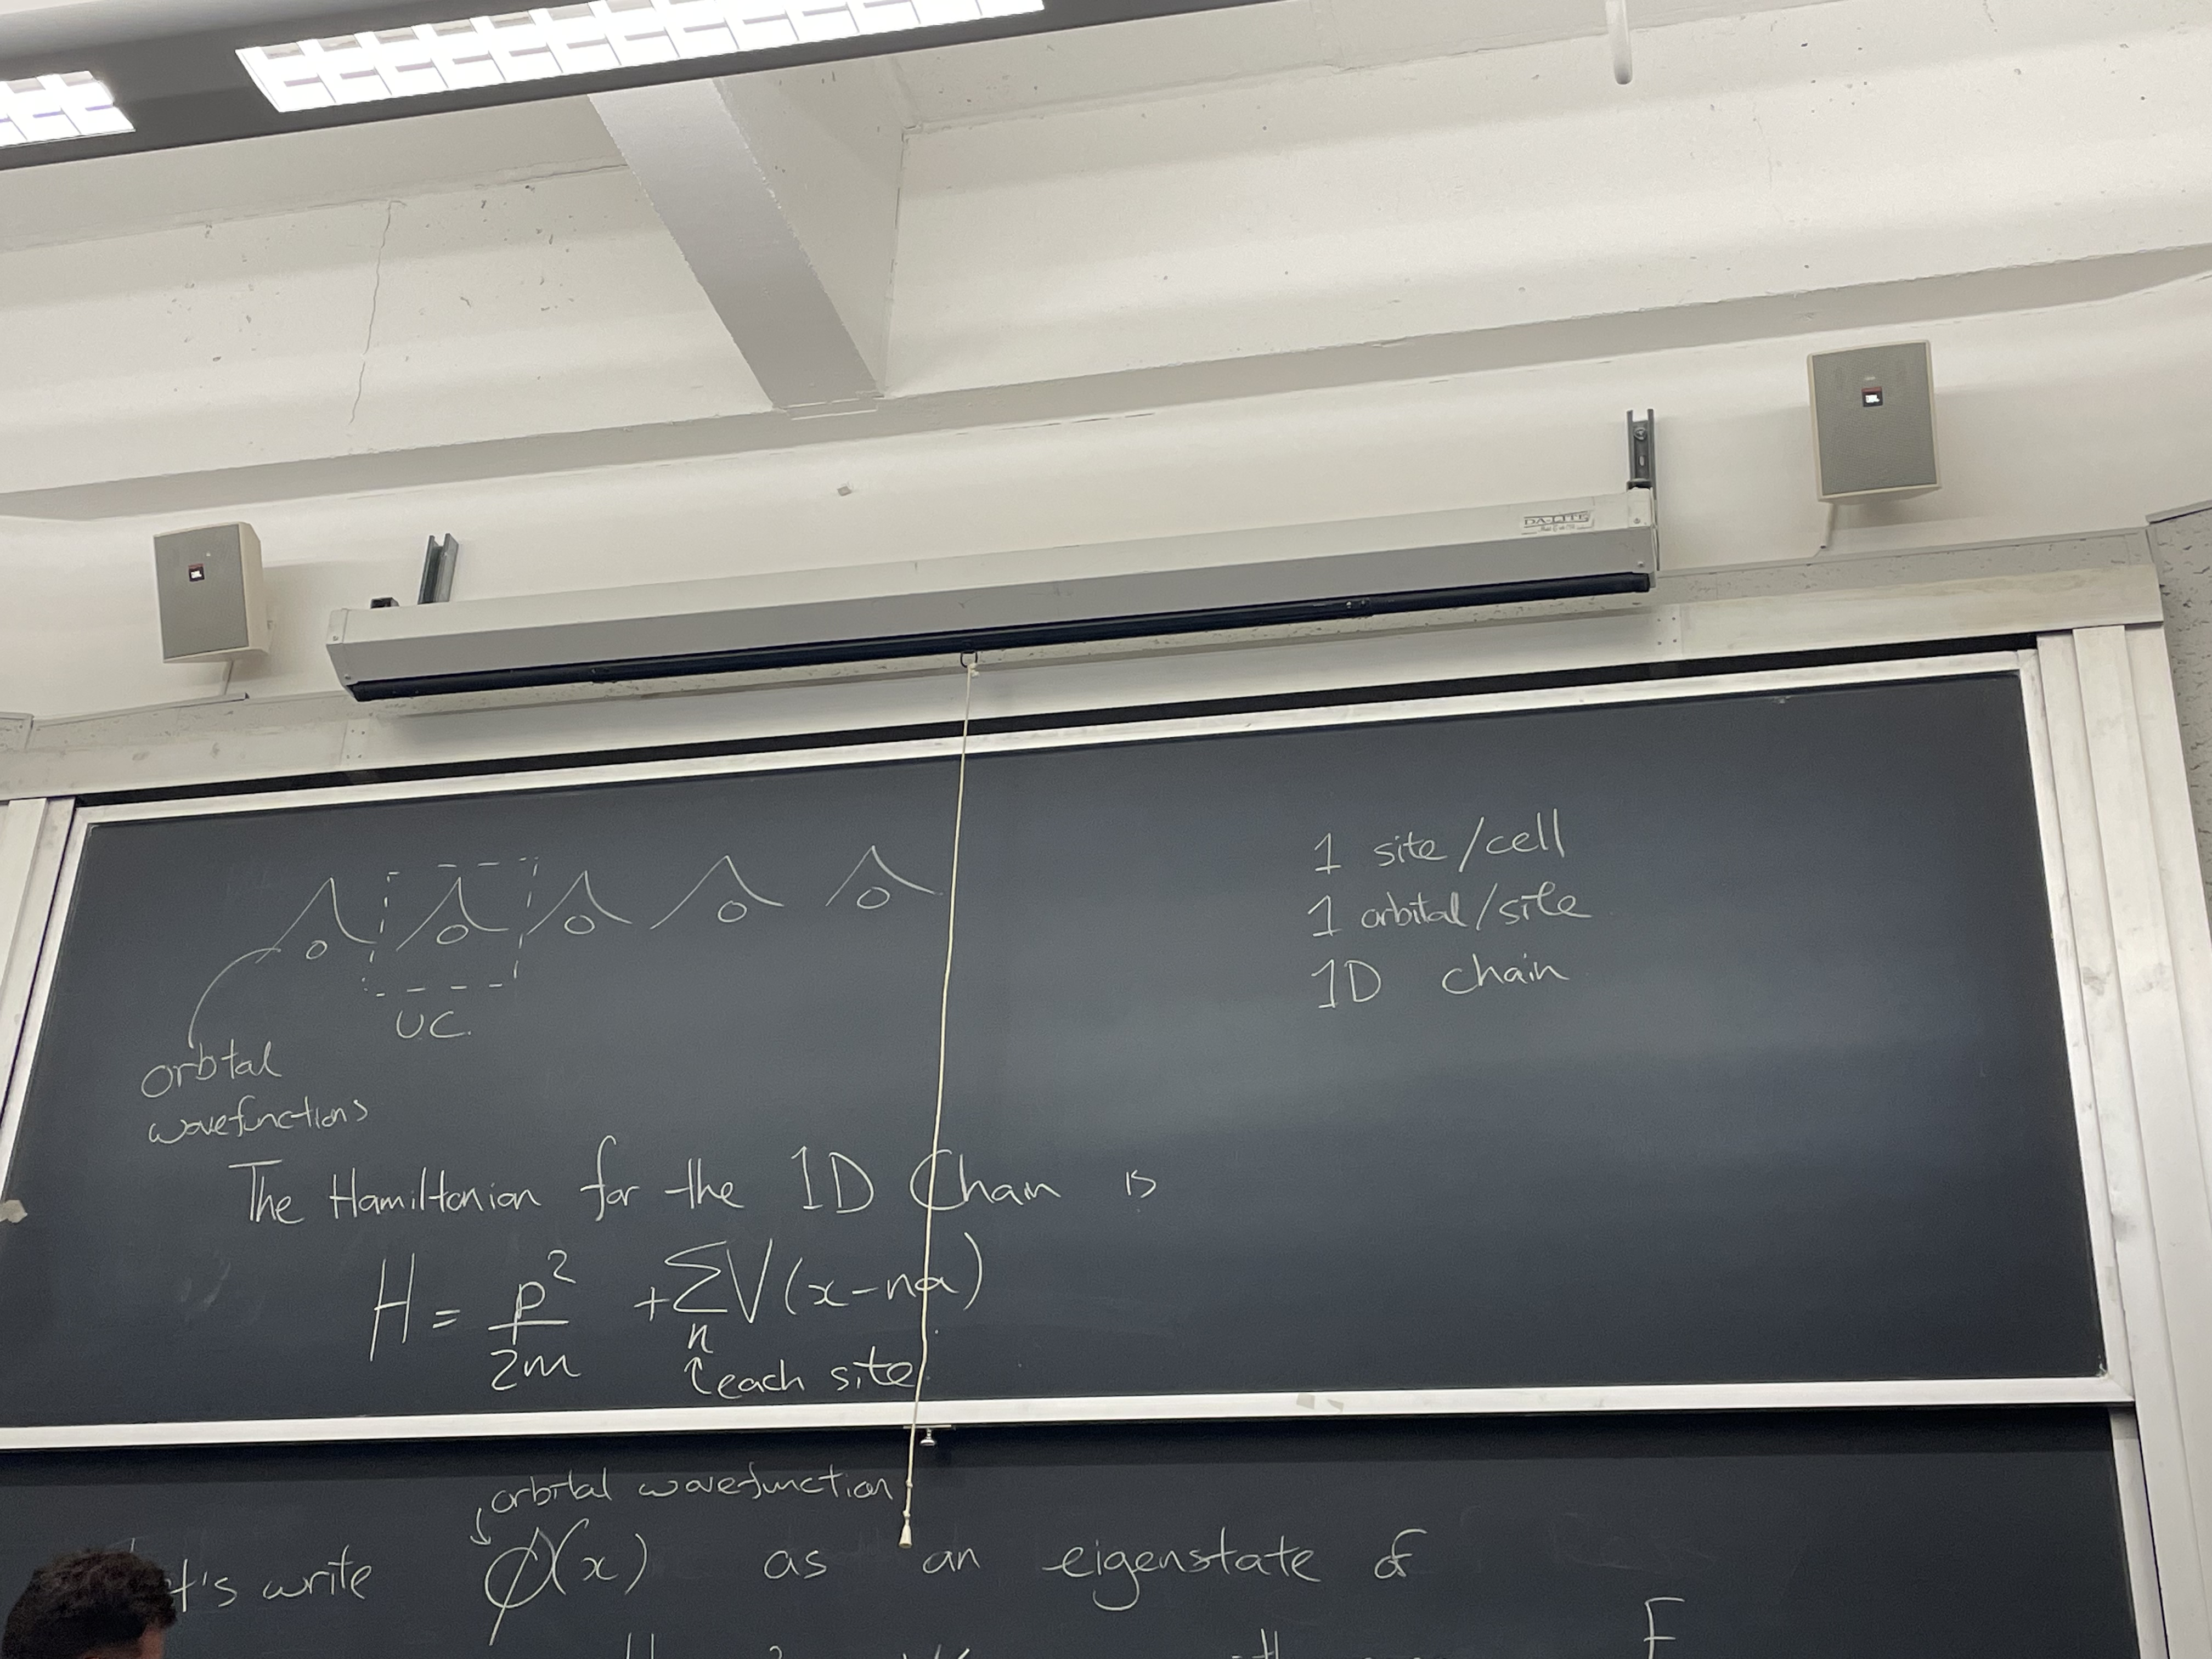
\includegraphics[scale=0.05]{Pictures/Jan 22/Tight-binding.png}
\end{center} The Hamiltonian for the 1D Chain is $$ H = \frac{\mathbf{p}^2}{2m} + \sum_{n} V(x-na) $$ Let $\phi(x)$ be the eigenstate of $$ H_0 = \frac{\mathbf{p}^2}{2m} + V(x) $$ with energy $E_0$ i.e. $\phi(x)$ is the \textbf{Orbital Wavefunction}. The Hilbert Space for the chain consists of one orbital at each site $\{\phi_n(x)\}_{n \in I}$ (the $n$ subscript labels the different sites) and the wavefunction for the chain is then $$ \boxed{\psi(x) = \sum_{n} c_n \phi_n(x - na)} $$ (linear combination of atomic orbitals) 

\vskip 1cm
\subsection{Review: Bloch's Theorem}
Next, we recall Bloch's theorem for a system with Translational Symmetry. Bloch's Theorem tells us that $$ \boxed{ \psi_k(x+a) = e^{ika} \psi_k(x) } $$ where $a$ is the size of the Unit Cell, which in this case is the distance between atoms \begin{note} {Add a proof} \end{note}.
\\
\\
From this, we can arrive at the conclusion that $$ c_n = c_0 e^{ikna} $$ and including the normalization, a chain of $N$ atoms is described by wavefunctions $$ \boxed{\psi_k(x) = \frac{1}{\sqrt{N}} \sum_{n} e^{ikna} \psi(x-na)  } $$ This can be interpreted as the single orbital wavefunction $\phi(x)$ being modulated by the free-electron wavefunction $e^{ikx}$.
\\
\\
The Energy Spectrum (or dispersion relation) is given by $$ E(k) = E_0 - 2t \cos(ka) $$ where $t$ is called the \textbf{Overlap integral} $$ t \equiv \int \mathrm{d}x ~ \phi(x) V(x) \phi(x-a) $$ \begin{center}
  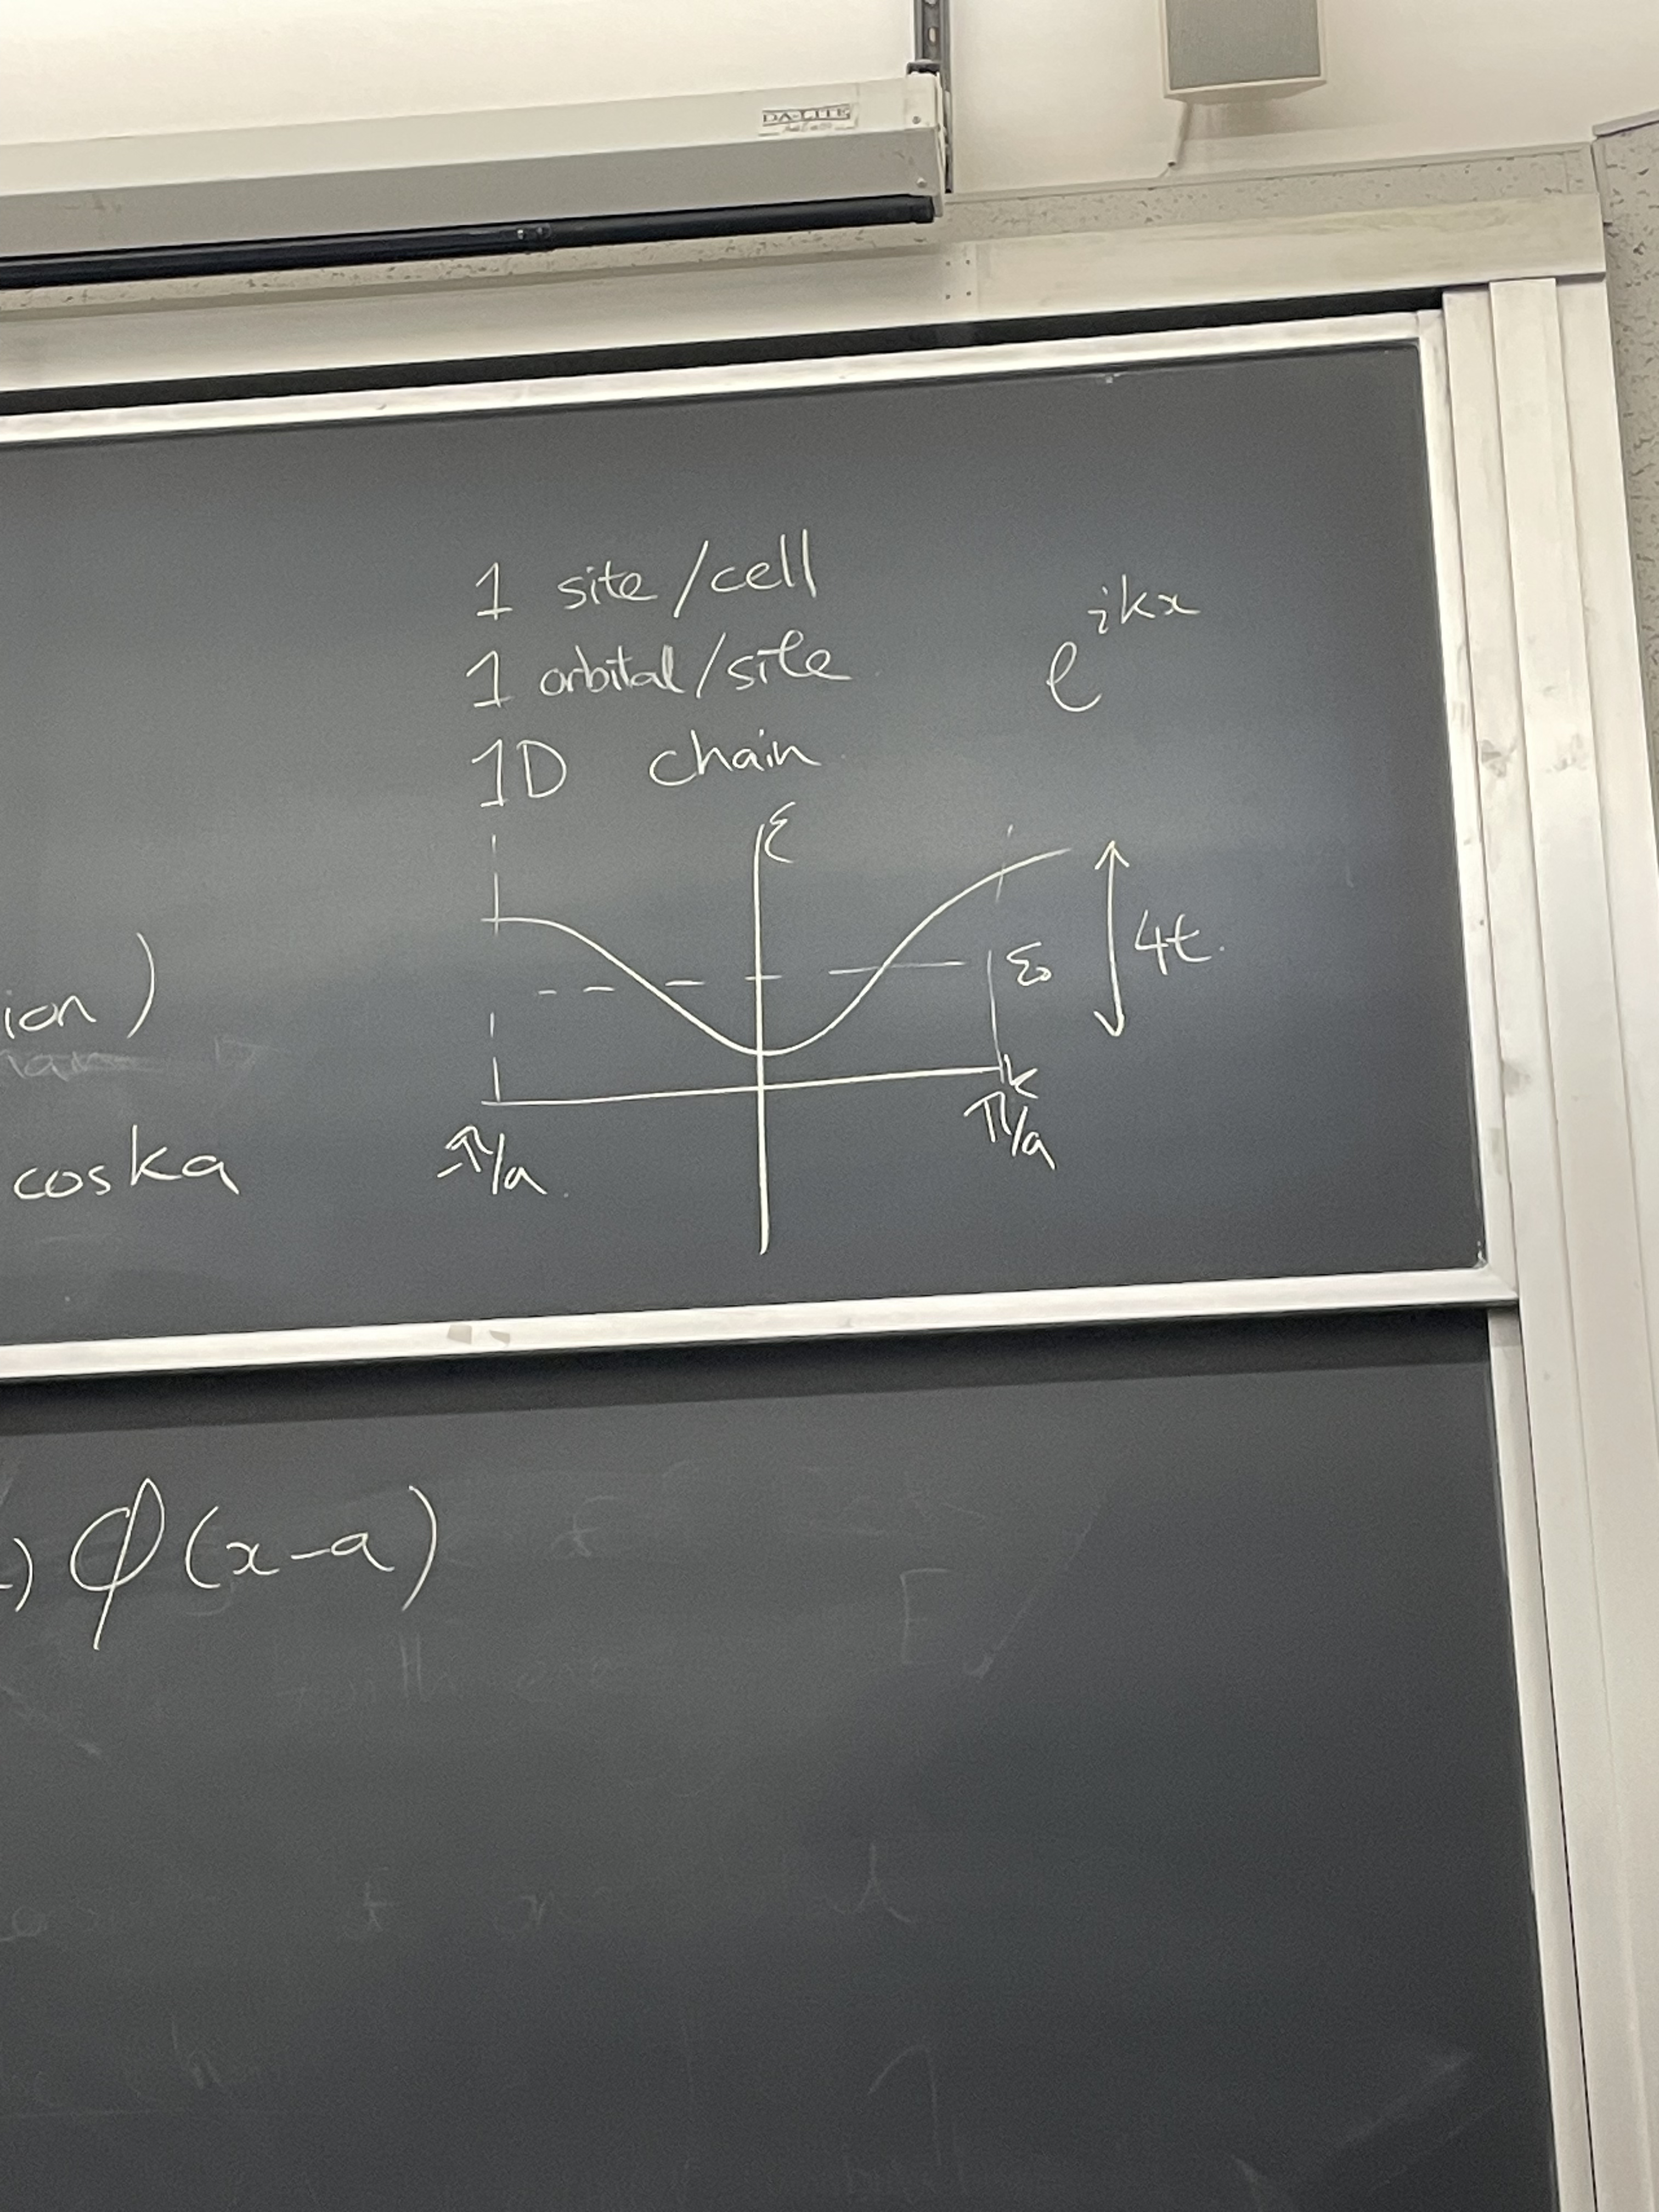
\includegraphics[scale=0.05]{Pictures/Jan 22/Tight-binding Dispersion.png}
\end{center} This model is too trivial to display any topological behavior. The physics we're interested in becomes apparent once we have \textbf{at least two bands \emph{and} a bandgap}. As our first case, we study the SSH model (Phys. Rev. Lett. 42 1698 (1979)).

\vskip 1cm
\subsection{SSH Model}
In the SSH model we, once again, have a 1D chain. However, this time, we have \textbf{two kinds of bonds} (alternating) with different overlap/hopping parameters $t_1, t_2$.
\begin{center}
  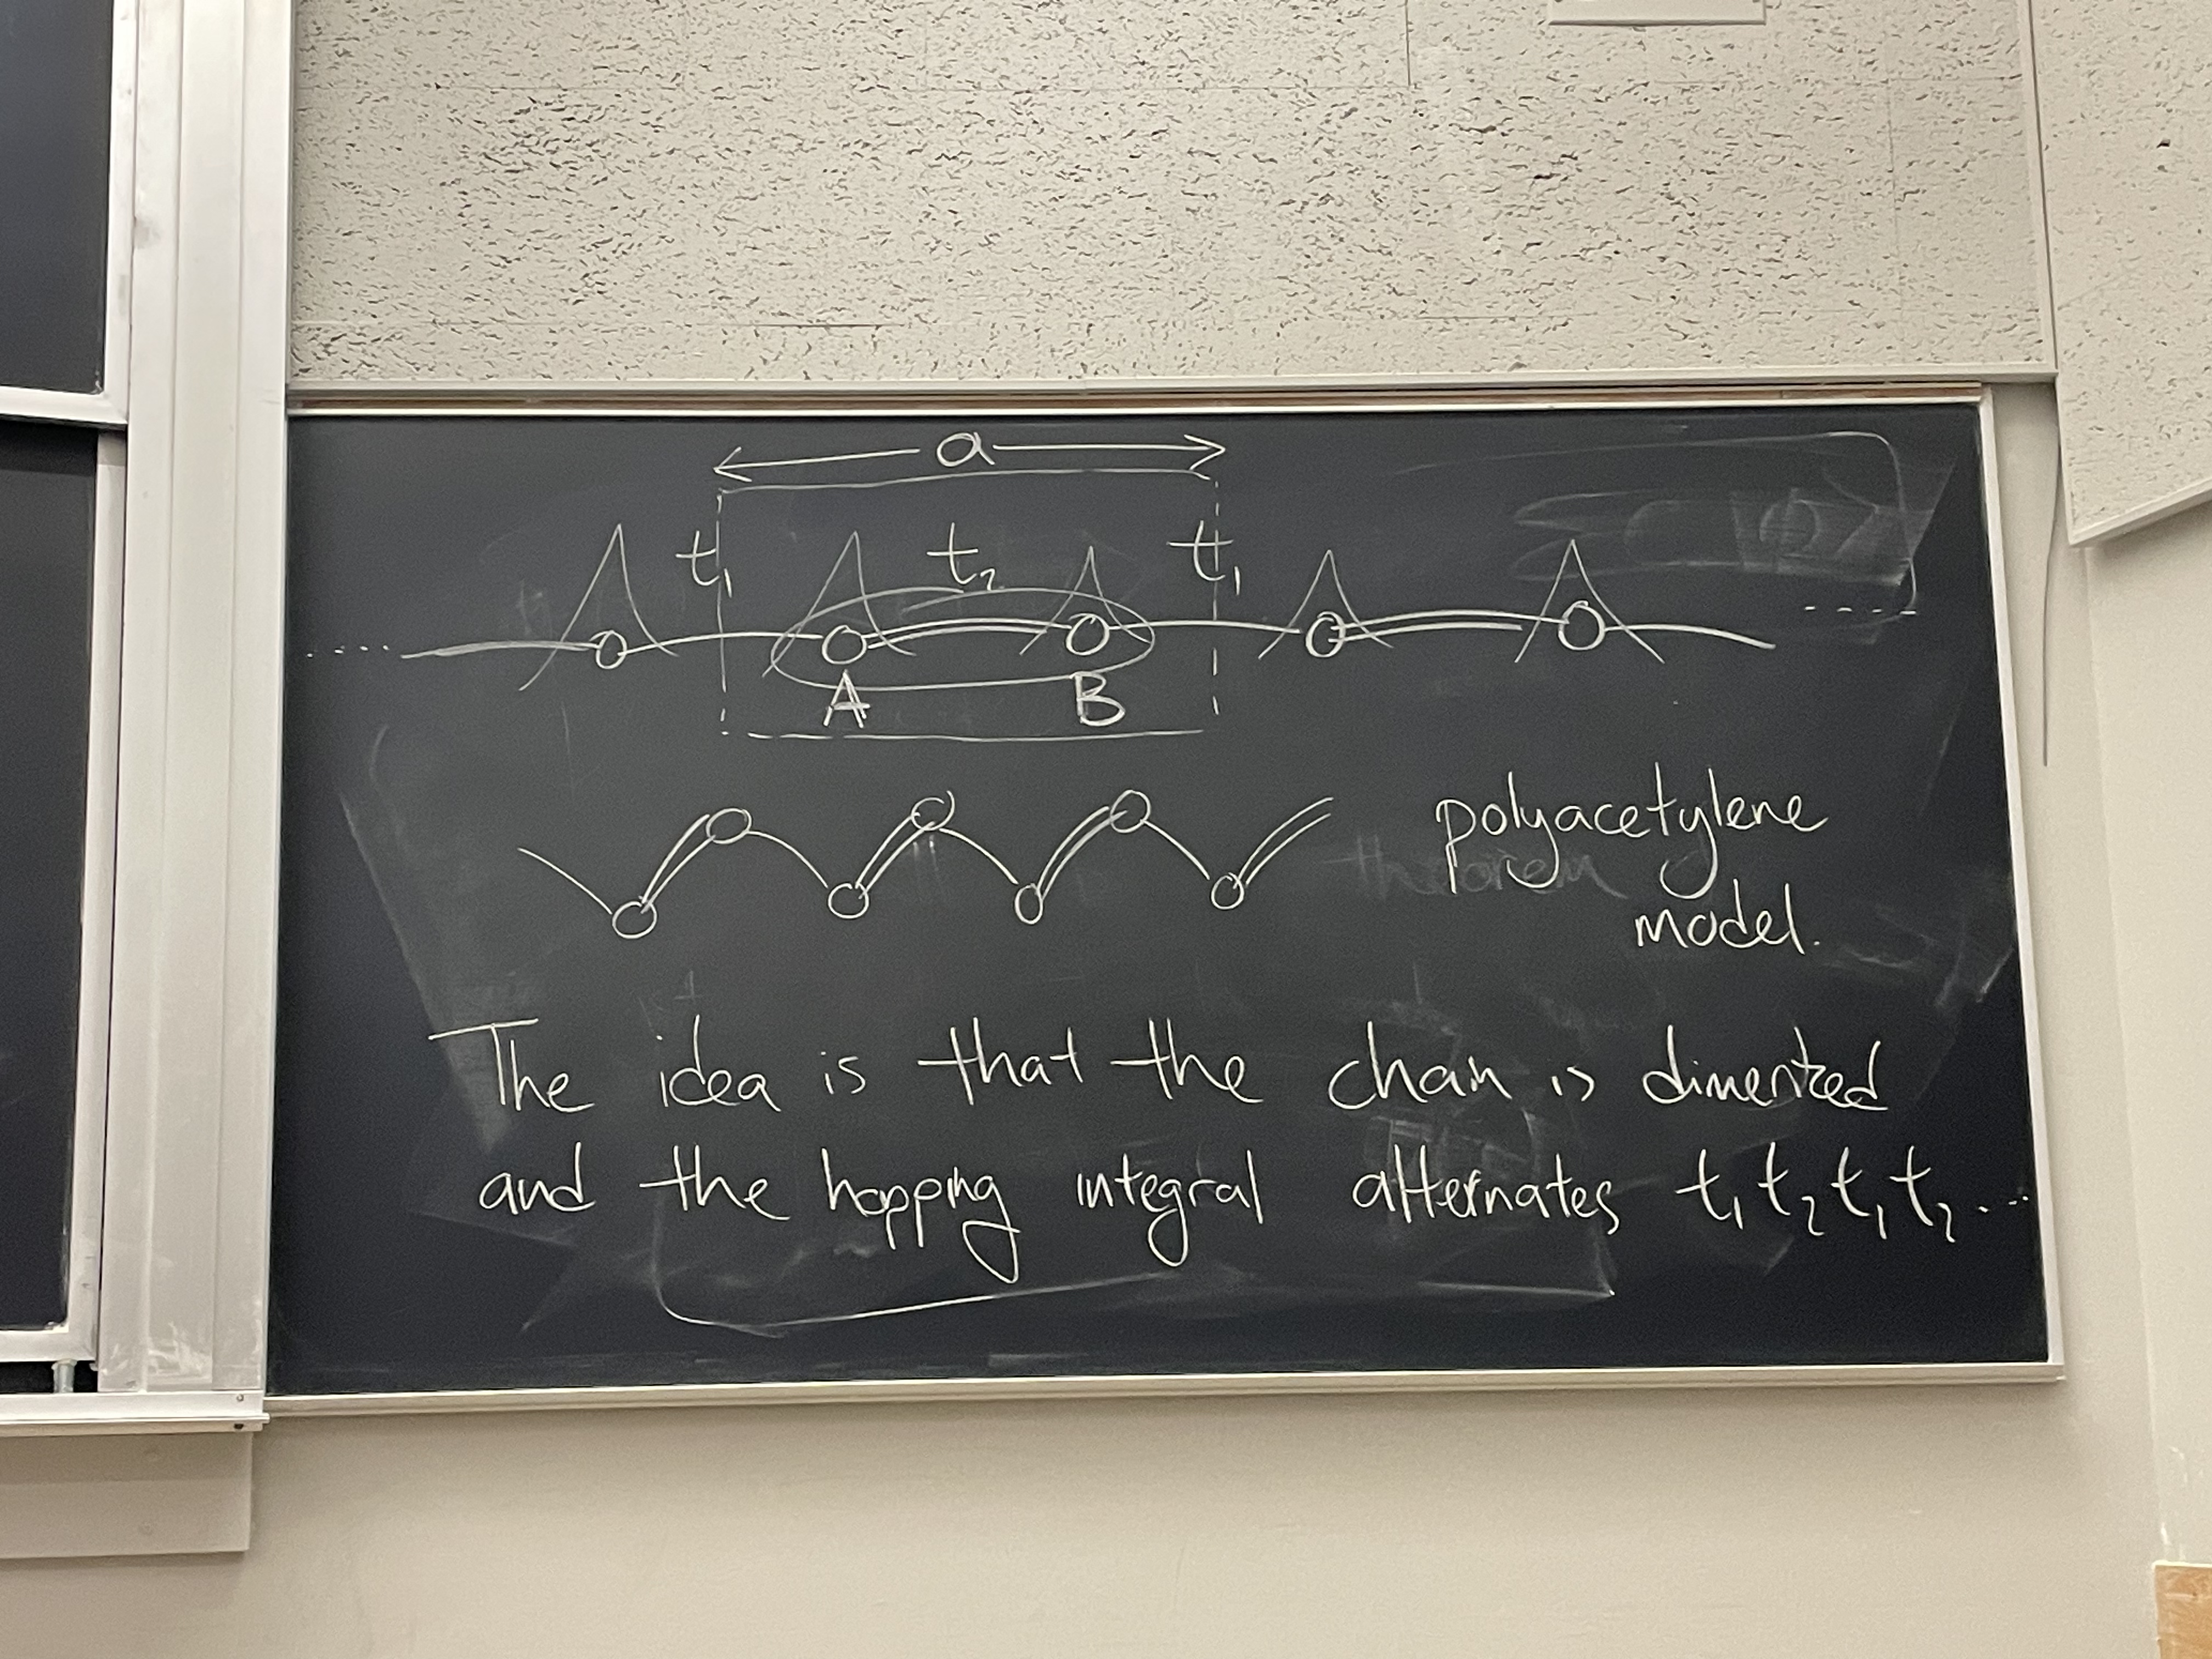
\includegraphics[scale=0.05]{Pictures/Jan 22/SSH Model.png}
\end{center}
For example, Polyacetylene is described by an SSH model. The idea is that the chain is \textbf{dimerised} because the hopping integral alternates.
\\
\\
The wavefunctions for this system are $$ \psi_k(x) = \frac{1}{\sqrt{N}} \sum_{n} e^{ikna} \left( \alpha_{k} \phi_{nA} + \beta_k \phi_{nB} \right) $$ where $a$ is the unit cell size and it is $2 \times$ the distance between sites. $\phi_{nA}, \phi_{nB}$ are the orbital waves on sites $A$ and $B$. 

\begin{redbox}
What are $\alpha_k, \beta_k$? \\
Probability amplitudes.
\end{redbox}

\begin{itemize}
  \item Now we need to solve the Schr\"odinger Equation to determine $\alpha_{k}$ and $\beta_k$. We know that $$ |\alpha_k|^2 + |\beta_k|^2  = 1 $$ 
  \item This is a 2D Hilbert Space
  \item We want to solve $H \psi_k(x) = E(k) \psi_k(x) $. To construct the matrix, take the product with $\bra{\phi_{nA}}$ and $\bra{\phi_{nB}}$, giving us the two equations 
  \begin{align*}
    \braket{\phi_{nA}}{H|\psi_k(x)} &= E(k) \braket{\phi_{nA}}{\psi_k} \\
    \braket{\phi_{nB}}{H|\psi_k(x)} &= E(k) \braket{\phi_{nB}}{\psi_k} \\
  \end{align*}

  \item Taking the first of these equations, the RHS is 
  \begin{align*}
    \braket{\phi_{nA}}{ \sum_{n'} e^{ikn'a} | \left( \alpha_k \phi_{n'A} + \beta_{k} \phi_{n'B} \right) }
  \end{align*} \begin{note}
    {missed a bit here}
  \end{note} So, the RHS is $E(k) \alpha_k e^{ikna} $

  \item Now, for the LHS, 
  \begin{align*}
    \sum_{n'} \braket{\phi_{nA}}{H|e^{ikn'a} \left(\alpha_{k} \phi_{n'A} + \beta_{k} \phi_{n' B}\right) } 
  \end{align*} 
  \item Recall that $H$ is described as $$ H = H_0 + \sum_{n'} V(x-n'a) $$ where $H_0 \ket{\phi_{n'A}} = E_0 $. When we take the inner product, only the $n=n'$ inner product survives when we dot with $H_0$, giving $$ \braket{\phi_{n'A}}{H_0|\left(\alpha_{k} \phi_{n'A} + \beta_{k} \phi_{n' B}\right)} = E_0 \alpha_k e^{ikna} $$
  \item The Second Term (only nearest neighbor hopping) is equal to 
  \begin{align*}
    &= e^{ikna} \braket{\phi_{nA}}{V_0(x-x_{n,B})| \beta_k \phi_{n,B} } + e^{ik(n-1)a} \braket{\phi_{nA}}{V_0(x-x_{n-1,B})| \beta_k \phi_{n-1,B} } \\
    &= \beta_k t_1 e^{ikna} + \beta_k t_2 e^{ik(n-1)a} \\
    &= \beta_k e^{ikna} \left( t_1 + t_2 e^{-ika} \right)
  \end{align*} 
\end{itemize}

%%%%%%%%%%%%%%%%%%%%%%%%%%%%%%%%%%%%%%%%%%%%%%%%
\pagebreak
\section{January 24, 2025:}
%%%%%%%%%%%%%%%%%%%%%%%%%%%%%%%%%%%%%%%%%%%%%%%%

Things get more interesting today. We won't reach the Topological aspects yet, but we'll cover them next Monday.
\\
\\
We left off looking at the LHS and RHS of the Schr\"odinger Equation for the SSH model, ending with the following equation: 
\begin{align*}
  &\alpha_k E_0 e^{ikna} + \beta_k t_1 e^{ikna} + \beta_k t_2 e^{ik(n-1)a} = \alpha_k E(k) e^{ikna} \\
  \implies& \alpha_k (E(k) - E_0) + \beta_k (t_1 + t_1 e^{-ika}) = 0 \\
\end{align*} Performing the same procedure, but taking the inner product with $\bra{\phi_{nB}}$ instead, we get a similar equation, giving us the following system of simultaneous equations:
\begin{align*}
  & \alpha_k (E(k) - E_0) + \beta_k (t_1 + t_1 e^{-ika}) = 0 \\ 
  & \beta_k (E(k) - E_0) + \alpha_k (t_1 + t_1 e^{+ika}) = 0 \\ 
\end{align*} For a 2D Hilbert Space (in this case, spanned by $\ket{\phi_{nA}}$ and $\ket{\phi_{nB}}$) we can regard the wavefunctions as "$S = 1/2$" \textbf{spinors} or "Pseudospins". 
\\
\\
Pseudospins or Spinors are objects of the form $$ \begin{pmatrix}
  \alpha_{k} \\ \beta_{k}
\end{pmatrix} $$ We can write these two simultaneous equations represented by this spinor as $$ \underbrace{\begin{pmatrix}
  E_0 & t_1 + t_2 e^{-ika} \\
  t_1 + t_2 e^{+ika} & E_0 \\
\end{pmatrix}}_{\text{"Bloch Hamiltonian"}} \begin{pmatrix}
  \alpha_k \\ \beta_k
\end{pmatrix} =  E(k) \begin{pmatrix}
  \alpha_k \\ \beta_k
\end{pmatrix} $$ where it's called the "Bloch Hamiltonian" because everything is represented in $k$-space. The Bloch Hamiltonian has the form $$ H(k) \underbrace{\vec{\phi}_k}_{\text{Spinor}} = E(k) \vec{\phi}_k $$ Generally, a Bloch Hamiltonian is an $N \times N$ matrix where $$ N = \begin{pmatrix}
  \text{\# sites} \\
  \text{per U.C.} \\
\end{pmatrix} \times \begin{pmatrix}
  \text{\# orbitals} \\
  \text{per site} \\
\end{pmatrix} \times \begin{pmatrix}
  \text{\# of} \\
  \text{dimensions} \\
\end{pmatrix}  $$ So, in our case, we have $N = 2 \times 1 \times 1 = 2$ We solve our $2 \times 2$ matrix in the usual way. 

\vskip 1cm
\subsection{What is the "Pseudospin" representation?}
The Pseudospin is the $2$-state system of each allowed value of momentum $k$.

\vskip 1cm
\subsubsection*{But what do $\alpha_k$ and $\beta_k$ represent?} 
\vskip 0.5cm
\begin{center}
  Include figure of B and A sublattices (blue and yellow)
\end{center} We visualize these as two interpenetrating sublattices. Basically, $\alpha$ and $\beta$ refer to the wavefunctions on the $A$ and $B$ sublattices respectively, but let's take this idea a little further.
\\
\\
Any $2 \times 2$ matrix can be represented as a linear superposition of Pauli matrices and the identity. 
\begin{align*}
  \text{Pauli Matrices:} ~ \sigma_x = \begin{pmatrix}
    0 & 1 \\
    1 & 0
  \end{pmatrix}, ~ \sigma_y = \begin{pmatrix}
    0 & -i \\
    i & 0
  \end{pmatrix}  ~ \sigma_z = \begin{pmatrix}
    1 & 0 \\
    0 & -1
  \end{pmatrix},  ~ \sigma_0 = \mathbf{1} = \begin{pmatrix}
    1 & 0 \\
    0 & 1
  \end{pmatrix}
\end{align*} Let us represent our Bloch Hamiltonian as 
\begin{align*}
  H(k) = \begin{pmatrix}
    E_0 & \Delta(k) \\
    \Delta^*(k) & E_0 \\
  \end{pmatrix}, ~ \Delta(k) = t_1 + t_2 e^{-ika}
\end{align*} Then, solving the Schr\"odinger Equation amounts to solving 
\begin{align*}
  &\mathrm{det} \begin{bmatrix}
    E_0 - E(k) & \Delta(k) \\
    \Delta^*(k) & E_0 - E(l)
  \end{bmatrix} = 0 \\
  \implies& E_0 - E(k) = \pm \left| \Delta(k) \right| \\
  \implies& \left| \Delta(k) \right| = \left| t_1 + t_2 e^{ika} \right| = \sqrt{t_1^2 + t_2^2 + 2t_1t_2 \cos(ka)}
\end{align*} 

\subsubsection*{The Band Structure}
For the sake of convenience let's set $E_0 = 0$. Now, we have 
\begin{align*}
  &k = 0 \implies \Delta(0) = |t_1 + t_2| \\
  &k = \frac{\pi}{a} \implies \Delta(\frac{\pi}{a}) = |t_1 - t_2| 
\end{align*}
\begin{center}
  Include figure of the Band Structure.
\end{center} Notice that the band structure just depends on $|t_1 - t_2|$ and so doesn't actually care which one is bigger. \begin{note}
  {Ask for clarification}
\end{note} \\
\\
Now that we have the Band Structure, let's get back to the psuedospin wavefunctions 
\begin{align*}
  &\Delta(k) = \underbrace{\Delta_1(k)}_{\mathrm{Re}(\Delta(k))} +  \underbrace{i\Delta_2(k)}_{\mathrm{Im}(\Delta(k))}
\end{align*} So 
\begin{align*}
  H(k) &= \begin{pmatrix}
    E_0 & \Delta_1 + i \Delta_2 \\
    \Delta_1 - i \Delta_2 & E_0 \\
  \end{pmatrix} = E_0 \begin{pmatrix}
    1 & 0 \\
    0 & 1
  \end{pmatrix} + \Delta_1 \begin{pmatrix}
    0 & 1 \\
    1 & 0
  \end{pmatrix} + \Delta_2 \begin{pmatrix}
    0 & i \\
    -i & 0
  \end{pmatrix} \\
  &= E_0 \mathbf{1} + \Delta_1 \sigma_x - \Delta_2 \sigma_{y} + 0 \sigma_z
\end{align*} Now, since we have $E_0 = 0$ we can write 
\begin{align*}
  H(k) &= \vec{\sigma} \cdot \vec{b}(k)
\end{align*}
where \begin{align*}
  &\vec{b}_x = \begin{pmatrix}
    \Delta_1(k) \\ 0 \\ 0
  \end{pmatrix}, ~\vec{b}_y = \begin{pmatrix}
    0 \\ \Delta_2(k) \\ 0
  \end{pmatrix}, ~\vec{b}_z = \begin{pmatrix}
    0\\ 0 \\ 0
  \end{pmatrix} \\
  \text{ and }& \vec{b}(k) = b_x \hat{x} + b_y \hat{y} + b_z \hat{z}
\end{align*} This looks a lot like a spin in a magnetic field, and so we identify $\vec{\sigma}$ as being our pseudospin or spinor and $\vec{b}(k)$ as being our "Zeeman" field.
\\
\\
Note that there is no $\vec{\sigma}_z$ component. This follows from the fact that  the orbitals on site $A$ and $B$ are the same, and we have only allowed nearest neighbor hopping. If we did not restrict to nearest neighbors, we'd need to have a third parameter, but we would also lose all topological properties of the model (we'll show this later).
\\
\\
Now, in our case, the Hamiltonian only consists of $\sigma_x, \sigma_y$ and we know the Pauli matrices anti-commute with each other. As a result, $\sigma_z$ anticommutes with the Hamiltonian $\{\sigma_z, H\} = 0 $.
\\
\\
This is actually a special case of when some unitary operator $\Theta$ actos on $H$ as $$ \Theta H \Theta^{\dagger} = -H $$ The existence of such a relationship implies for $H \ket{\psi} = E\ket{\psi}$. that there exists another eigenstate with energy $-E$.  
\\
\\
This is a kind of \textbf{Chiral} symmetry, and such symmetries have very special consequences for the eigenvalues and are intimately related to the Topology in such systems.


% %%%%%%%%%%%%%%%%%%%%%%%%%%%%%%%%%%%%%%%%%%%%%%%%
% \pagebreak
% \section{ }
% %%%%%%%%%%%%%%%%%%%%%%%%%%%%%%%%%%%%%%%%%%%%%%%%


\end{document}









